
\section{Coalescence theory}

\begin{frame}{Intended Learning Outcomes}

        \underline{Coalescence theory}

	\bigskip

        In this lecture you will learn to
	\begin{itemize}
                \item describe principles and assumptions of the coalescence theory
                \item discuss the infinite sites model
                \item provide estimators of $\theta$ and effective population size
                \item measure genetic variability with summary statistics and the site frequency 
		spectrum with \texttt{R}
        \end{itemize}

\end{frame}


\begin{frame}{Motivation}

	\begin{figure}
                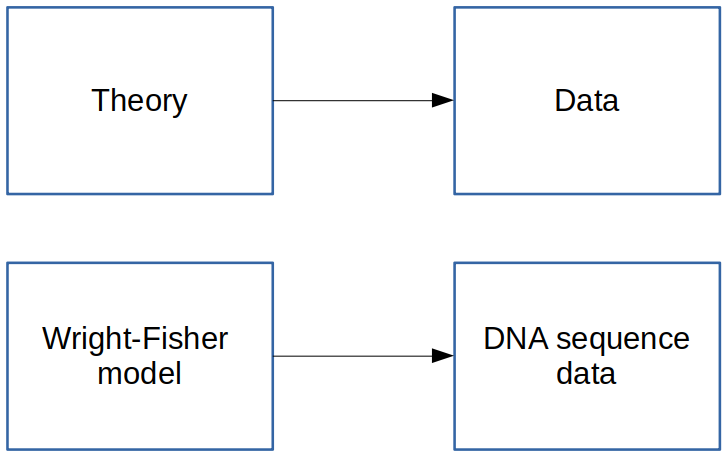
\includegraphics[width=0.7\textwidth]{Pics/data_theory}
        \end{figure}

\end{frame}


\begin{frame}{Motivation}

	e.g. on the X chromosomes, two Europeans differ, on average, in $0.08\%$ of sites, while
	individuals from African populations differ in $0.012\%$ of sites.

	\bigskip

	What do these numbers tell us \textit{about} the two populations?

	\pause

	\begin{block}{}
	We use \textbf{coalescence theory}, which is based on Wright-Fisher model, to consider the genealogy history
	of a sample and make inferences about populations instead of modelling changes of allele frequencies forward in time.
	\end{block}


\end{frame}


\begin{frame}{Coalescence}

	\begin{figure}
                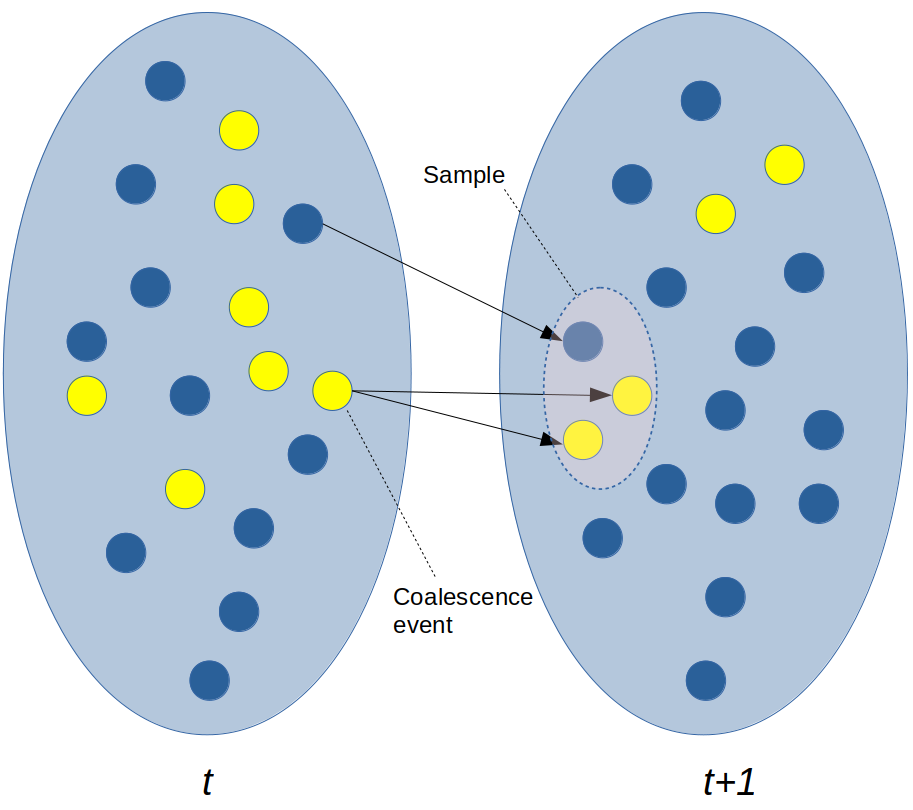
\includegraphics[width=0.5\textwidth]{Pics/coalescence} \
		\caption{Tracking the ancestry of a sample between two generations.}
        \end{figure}

\end{frame}


\begin{frame}{Coalescence}

	If two individual gene copies have the same parent in the previous generation, we say that the \textbf{ancestral lineage}
	representing these two individuals have \textbf{coalesced}.

	\bigskip

	They have a \textbf{common ancestor} and a \textbf{coalescent event} has occured.

\end{frame}


\begin{frame}{Coalescence tree}

        \begin{figure}
                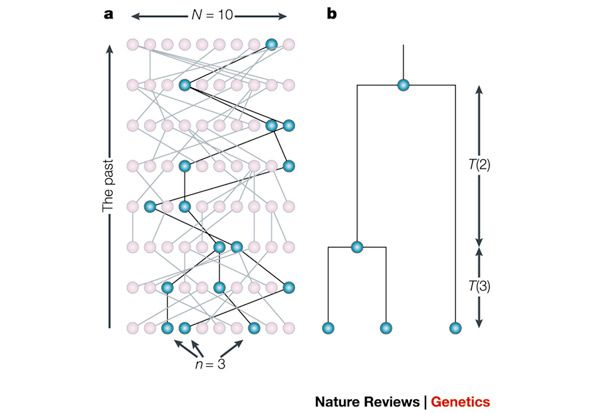
\includegraphics[width=0.7\textwidth]{Pics/coal_tree} \
                \caption{Ancestry of three samples.}
        \end{figure}

\end{frame}


\begin{frame}{Coalescence tree}

	The ancestry of an individual gene copy is represented by a line (or edge).

	\bigskip
	\begin{block}{}
	The time until two lineages find a \textbf{most recent common ancestor (MRCA)} is called \textbf{coalescence time}.
	\end{block}

	How can we find the coalescence time?

\end{frame}


\begin{frame}{Coalescence in a sample of two gene copies}

	As there are $2N$ potential parents "chosen" with equal probability, the probability of two individuals having the same
	parent in the previous generation is \pause $1/(2N)$.

	\bigskip

	The probability that two gene copies did NOT have the same parent in the previous generation is \pause $1-1/(2N)$.

	\bigskip

	The probability that two gene copies did not have the same parent in the past $r$ generations is \pause $[1-1/(2N)]^r$.

\end{frame}


\begin{frame}{Coalescence in a sample of two gene copies}

	The probability of not finding any common ancestor in generation $r-1$ but then finding the first common ancestor
	in generation $r$ is \pause
	\begin{equation}
		Pr(\texttt{...}) = [1-1/(2N)]^{r-1}[1/(2N)]
	\end{equation}

	\small

	This equation gives us the probability distribution of the time to the MRCA in a sample if size $n=2$. This is 
	a geometric random variable: the probability distribution of the number of Bernoulli trials needed to get one success.

	\bigskip
	\tiny
	jupyter-notebook: coalescence

\end{frame}


\begin{frame}{Coalescence in large populations}

	\begin{itemize}
		\item If we consider the limit of an infinitely large population, calculations 
		simplify but we can still 
		consider the effect of genetic drift.
		\item It is convenient to measure time in $2N$ generations, by setting $r=2Nt$ with $t$ measuring time in $2N$ generations.
	\end{itemize}

	\pause
	The probability that two gene copies do not find a common ancestor in $2Nt$ generations becomes
	\begin{equation*}
		[1-1/(2N)]^{2Nt} \rightarrow e^{-t} \texttt{ as } N \rightarrow \infty
	\end{equation*}


\end{frame}


\begin{frame}{Coalescence in large populations}

	As $N$ becomes large, the distribution of the coalescence times follows an \textbf{exponential distribution} with mean 1.

	\bigskip

	As time is measured in $2N$ generations, the mean (expected) time to coalescence is actually $2N$ generations.
	In other words, there is a constant rate of coalescence of $1$ per $2N$ generations.
	
	\bigskip
	\tiny
        jupyter-notebook: coalescence

\end{frame}


\begin{frame}{Coalescence in large population}

	\begin{itemize}
		\item The random process of following the lineages backward in time until a most recent common ancestor
		has been found is called a \textbf{coalescence process}.
		\item It is intuitive to understand that the expected coalescence time is $2N$ generations, although
		there is considerable variability in the coalescence times.
	\end{itemize}

\end{frame}


\begin{frame}{Coalescence in large population}

        \begin{itemize}
		\item The coalescence process in a large randomly mating diploid population with two sexes is the same as that
		in the simple haploid model.
		\item Once we have a conveniente description of the geneaology, then it is easy to derive various properties
		of our sample.
	\end{itemize}

\end{frame}


\begin{frame}{Genetic variability and population size}

	\begin{columns}

                \column{0.4\textwidth}

                \begin{figure}
                        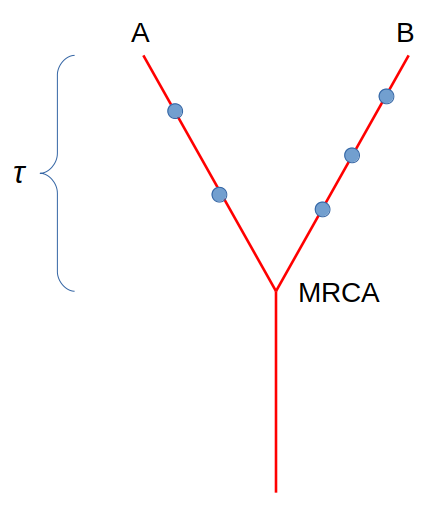
\includegraphics[width=0.9\textwidth]{Pics/tau}
                \end{figure}

                \column{0.6\textwidth}
          

		We expect $2N\mu t$ mutations on a lineage of length $t$. 

		Since $E[t]=1$ and there are two lineages,
		the expected number of mutations separating two gene copies is
		\begin{equation}
			\theta = 4N\mu
		\end{equation}
		which is a simple relationship between the amount of genetic variability and population sizes.

        \end{columns}

\end{frame}


\begin{frame}{Genetic variability and population size}

        \begin{columns}

                \column{0.4\textwidth}

                \begin{figure}
                        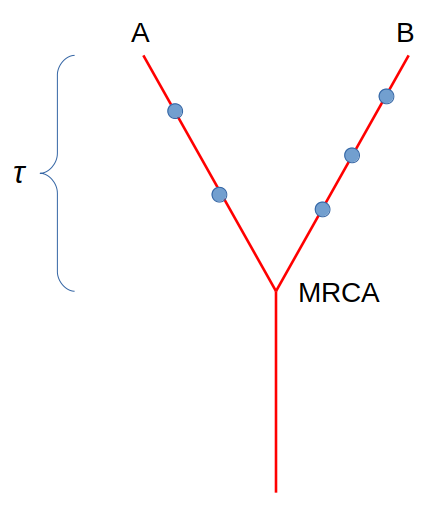
\includegraphics[width=0.9\textwidth]{Pics/tau}
                \end{figure}

                \column{0.6\textwidth}
 
		The expected number of mutations occuring in a lineage during any time interval of length $\tau$ is 
		$2N\mu\tau=\tau \theta /2$.

		\bigskip
		\small

		As such, we can think of the data generated by a coalescence process producing a coalescence tree and a 
		subsequent process in which mutations are distributed across the lineage of the tree at rate $\theta /2$.

        \end{columns}

\end{frame}


\begin{frame}{Infinite Sites Model}

	\begin{block}{}
		Each new mutation creates a new variable site, i.e. that each new mutation hits a new site in the sequence, such that no site experiences more than one mutation.
	\end{block}

	\bigskip

	\begin{figure}
        	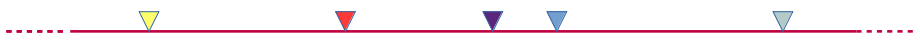
\includegraphics[width=0.9\textwidth]{Pics/iam} \\
		\caption{\small The sequence is infinitely long so that the chance of two mutations hit the same site is essentially zero.}
        \end{figure}

\end{frame}


\begin{frame}{Infinite Sites Model}

	The sites in which some of the individuals differ are called
	\textbf{segregating sites} or \textbf{single nucleotide polymorphisms} (SNPs).

 	\begin{figure}
                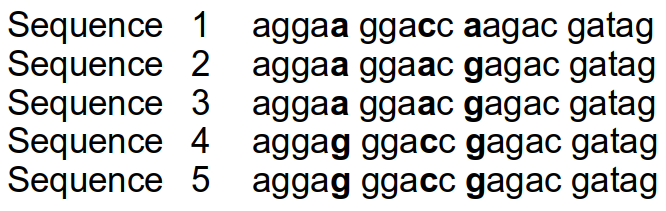
\includegraphics[width=0.7\textwidth]{Pics/sequences} 
        \end{figure}

	Under the infinite sites model, we can deduce which mutations occurred
	in the ancestry of a sample of sequences.

\end{frame}


\begin{frame}{Infinite Sites Model}

	The model does not distinguish between different nucleotides and does
        not care about invariable sites.

	\begin{figure}
                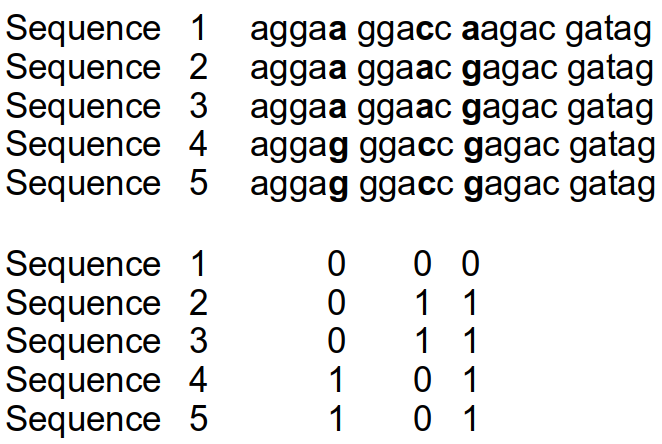
\includegraphics[width=0.5\textwidth]{Pics/sequences01} \\
		\caption{\small Data as a binary matrix of the variable sites.}
        \end{figure}

\end{frame}


\begin{frame}{Infinite Sites Model}

	\begin{itemize}
		\item Labelling with zeros and ones is arbitrary.
		\item Good approximation if the rate of mutation is low.
		\item DNA sequences with different mutations are different \textbf{haplotypes}.
	\end{itemize}

	\begin{figure}
                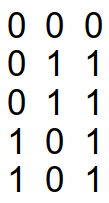
\includegraphics[width=0.1\textwidth]{Pics/sequences01_only} \\
		\caption{How many DNA sequences? How many haplotypes?}
        \end{figure}

\end{frame}


\begin{frame}{Tajima's estimator}

	We want an estimate of $\theta=4N\mu$ under the infinite sites model from the expected number of
	mutations separating two individuals based on the DNA sequences obtained from data.

	\pause
	\bigskip

	Data can be summarised as the \textbf{average number of pairwise differences}, or $\pi$.
	\begin{equation}
		\pi = \frac{\sum_{i<j}d_{i,j}}{n(n-1)/2}
	\end{equation}
	with $n$ sequences, $d_{i,j}$ number of differences between sequence $i$ and $j$.

\end{frame}


\begin{frame}{Tajima's estimator}

	\begin{figure}
                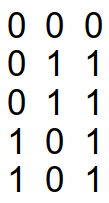
\includegraphics[width=0.1\textwidth]{Pics/sequences01_only} \\
		\caption{What is the value of $\pi$?}
        \end{figure}

	\pause
	$\pi = (2+2+2+2+0+2+2+2+2+0)/(5x4/2)=1.6$

\end{frame}


\begin{frame}{Tajima's estimator}

	\begin{columns}

                \column{0.3\textwidth}

                \begin{figure}
                        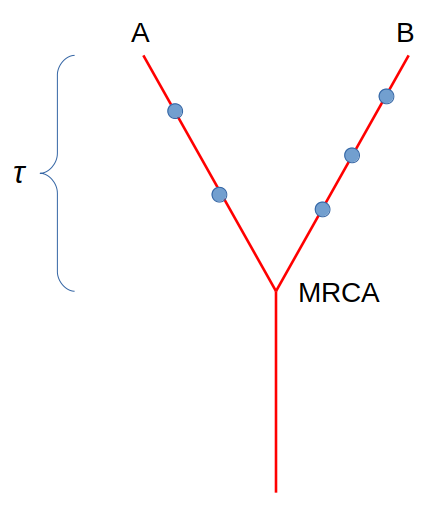
\includegraphics[width=0.9\textwidth]{Pics/tau}
                \end{figure}

                \column{0.7\textwidth}

		The expected number of nucleotide differences between two sequences is the expected 
		number of mutations, $\theta=4N\mu$.

		\begin{equation}
			E[d_{i,j}] = \theta
		\end{equation}

		\begin{equation}
			E[\pi] = \theta
		\end{equation}

		$\hat{\theta}_T = \pi$ is called \textbf{Tajima's} estimator of $\theta$.

        \end{columns}

\end{frame}


\begin{frame}{Effective population size}

	\begin{block}{}
		The number of individuals in a Wright-Fisher model that would produce the same amount of
		genetic drift as in the real population.
	\end{block}

	The amount of genetic drift can be measured as
	\begin{itemize}
		\item the expected heterozygosity
		\item expected number of pairwise differences
		\item rate of coalescence
		\item ...
	\end{itemize}

\end{frame}


\begin{frame}{Effective population size ($N_e$)}

	\textit{e.g. "A population with an effective size of 200 with respect to heterozygosity harbours
	the same amount of heterozygosity as a Wright-Fisher population of 200 individuals."}

	\bigskip

	The true number of individuals in the population can be very different from its effective
	population size!

\end{frame}


\begin{frame}{Effective population size}

	\begin{figure}
        	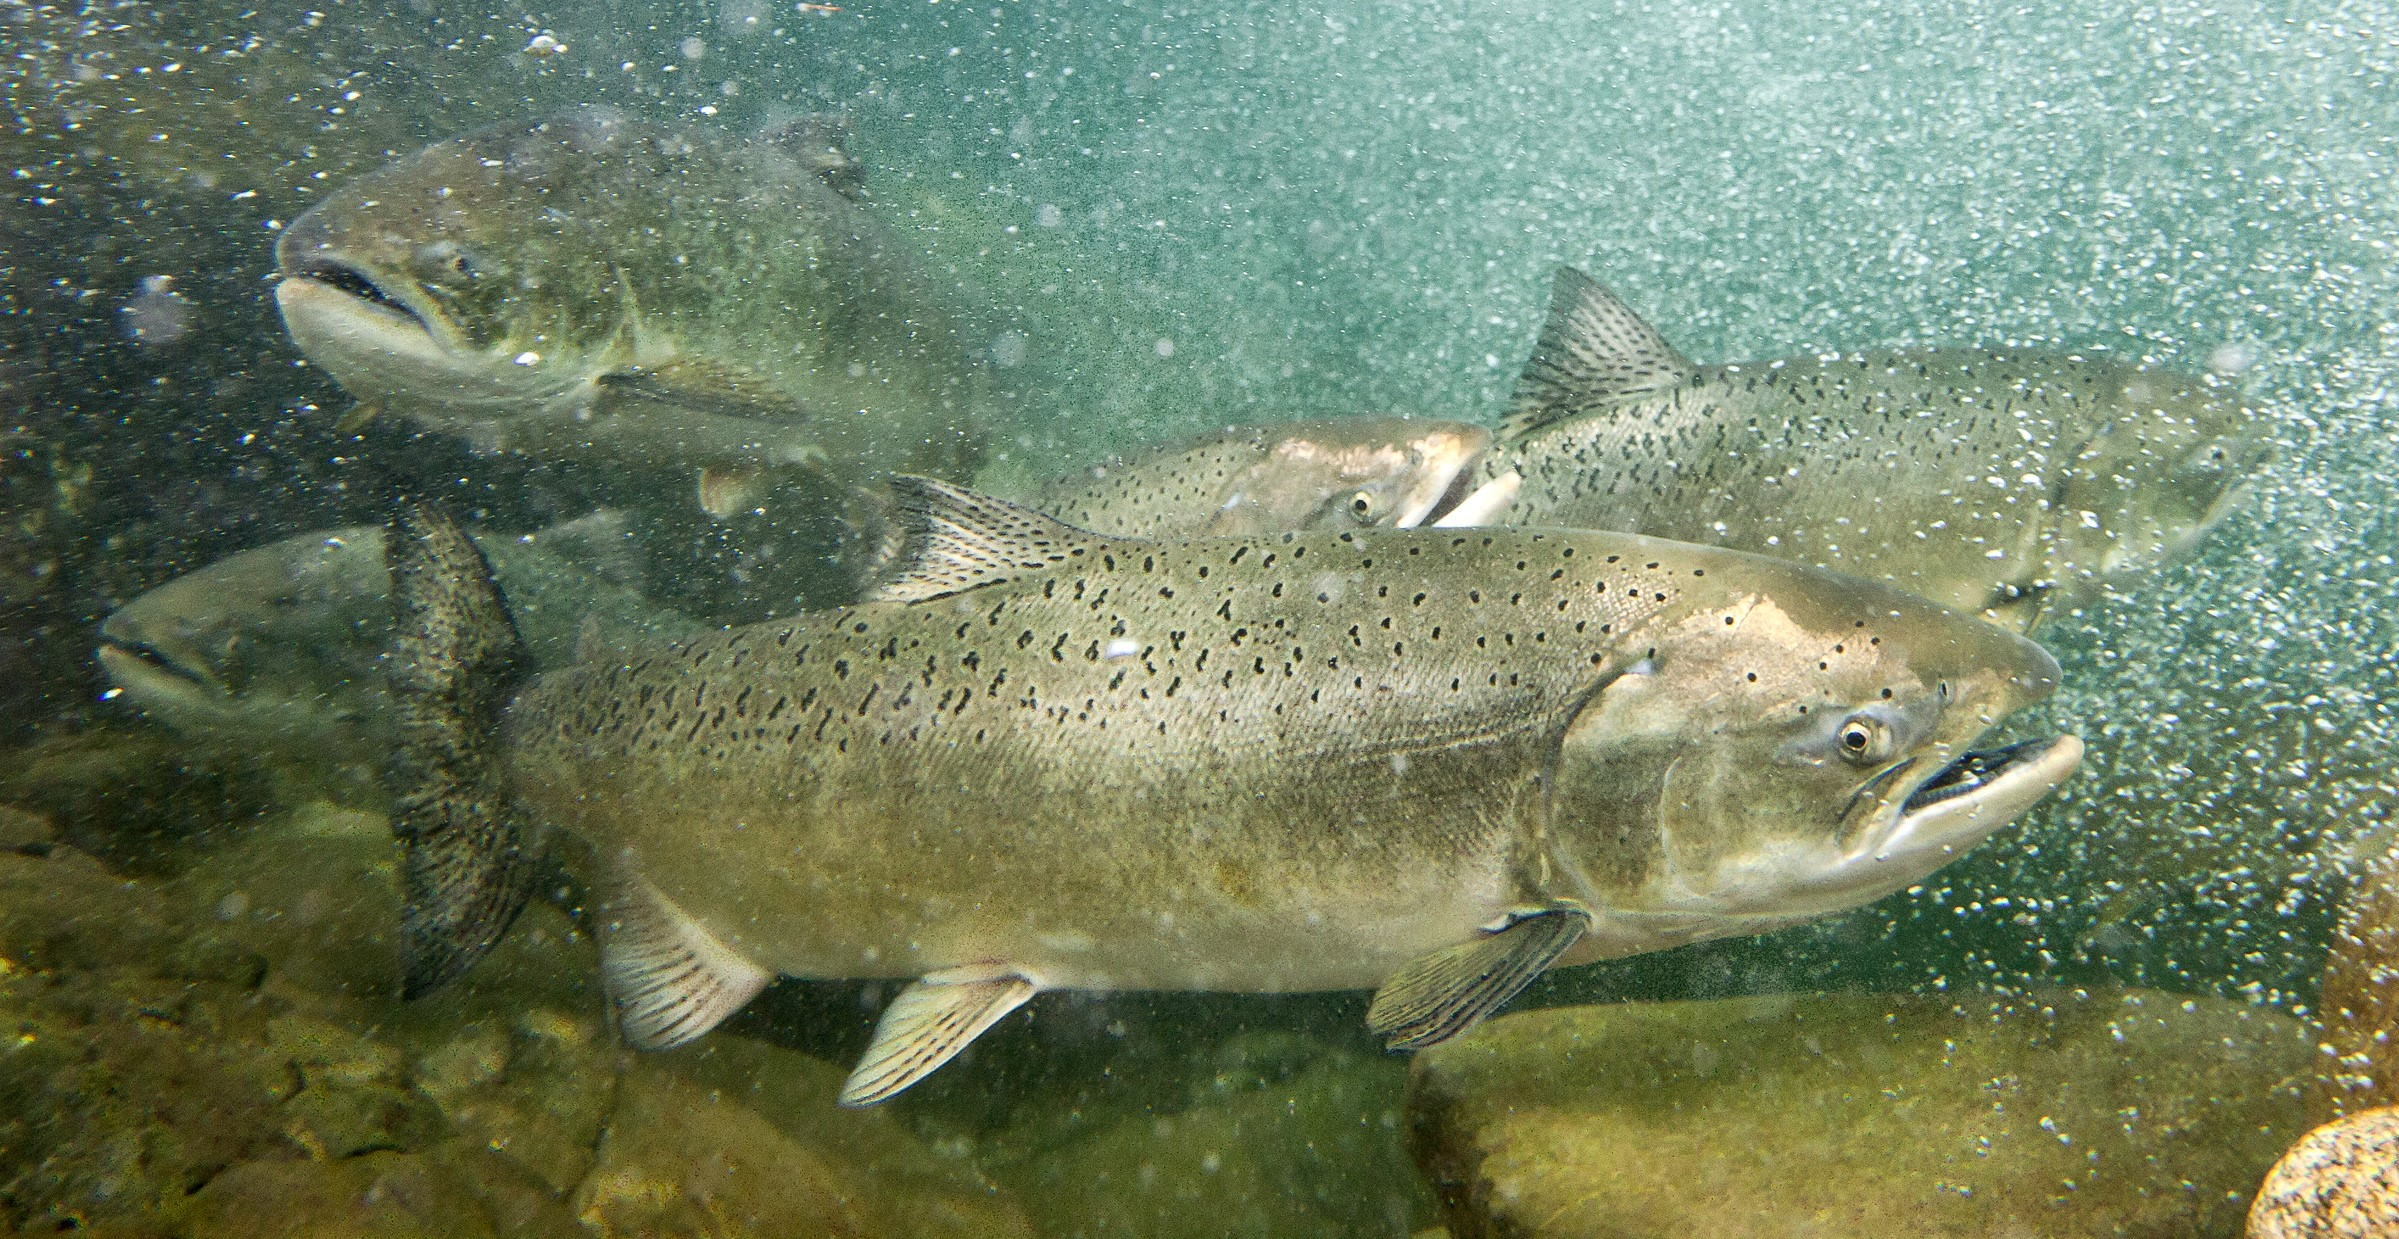
\includegraphics[width=0.7\textwidth]{Pics/salmon} \\
		\caption{The effective population size of the Chinook salmon (\textit{Oncorhynchus tshawytscha}) 
	  	has been estimated to be very low, possibly because the population size fluctuates between years and high variance
	  	offspring.} 
        \end{figure}

\end{frame}


\begin{frame}{Effective population size ($N_e$)}

	\begin{figure}
                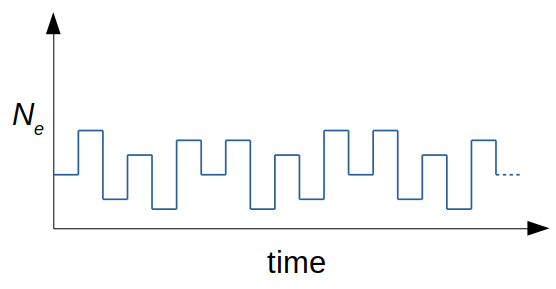
\includegraphics[width=0.4\textwidth]{Pics/ne_change}
	\end{figure}

	\small

	If a population fluctuates between sizes $N_1$, $N_2$, ..., $N_k$ at a proportion $p_1$, $p_2$, ..., $p_k$
	of the time, the coalescent effective population size is the harmonic mean:
	\begin{equation}
		N_e = \frac{1}{p_1/N_1 + p_2/N_2 + ... p_k/N_k}
	\end{equation}
	which is smaller that the arithmetic mean and gives more weight to smaller sizes.


\end{frame}


\begin{frame}{Effective population size ($N_e$)}

	\begin{figure}
                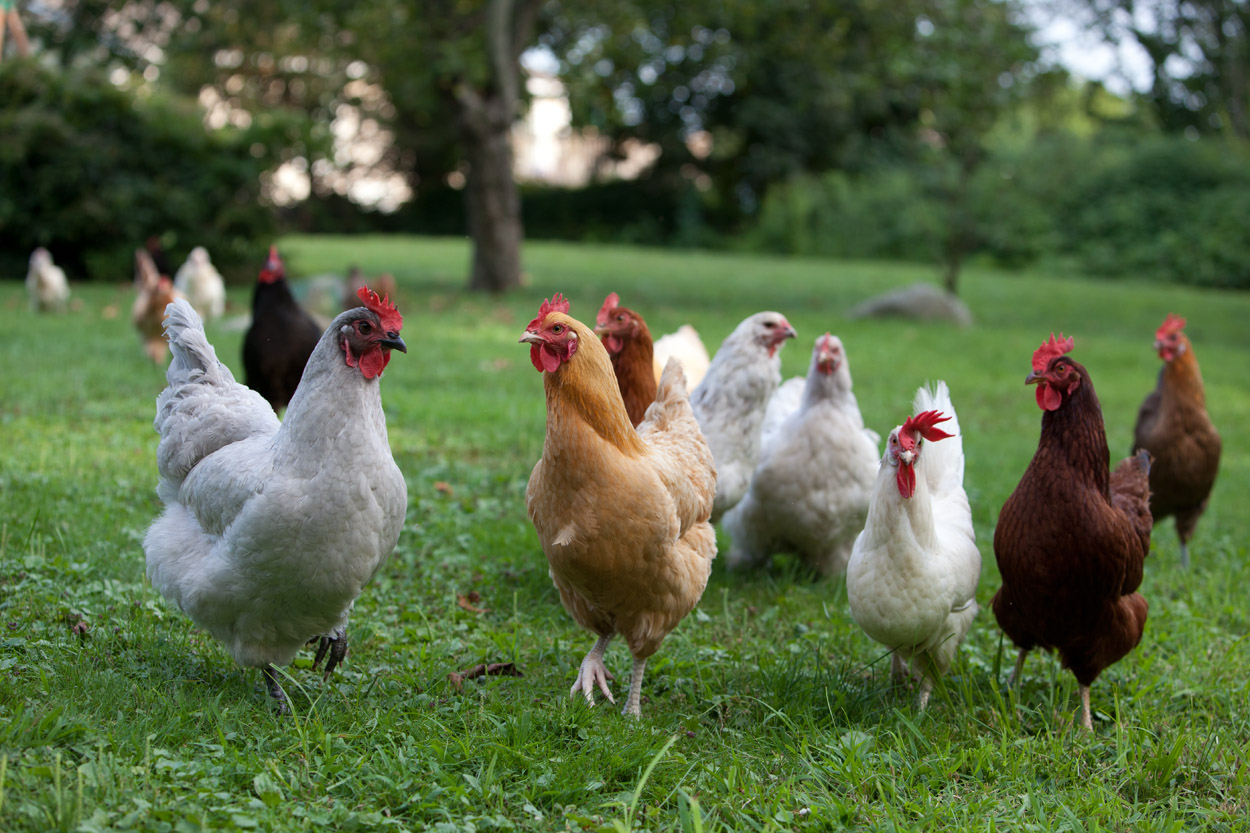
\includegraphics[width=0.4\textwidth]{Pics/chickens}
        \end{figure}

	The effective population size with unequal sex ratio is
	\begin{equation}
		N_e = \frac{4N_mN_f}{N_m+N_f}
	\end{equation}
	which is smaller than $N_m+N_f$.

\end{frame}


\begin{frame}{Interpreting estimates of $\theta$}

	\begin{table}[h]
                \centering
                \begin{tabular}{p{0.2\textwidth} p{0.7\textwidth}}
                        \toprule
                        \multicolumn{2}{p{0.9\textwidth}}{$\pi$ on autosomes} \\
                        \midrule
                        Mandenka    & 0.00120 \\
                        Biaka       & 0.00121 \\
			San & 0.00126 \\
                        Han & 0.00081 \\
			Basque & 0.00087 \\
			Melanesians & 0.00078 \\
                        \bottomrule
                \end{tabular}
        \end{table}

\end{frame}


\begin{frame}{Interpreting estimates of $\theta$}

        \begin{table}[h]
                \centering
                \begin{tabular}{p{0.2\textwidth} p{0.7\textwidth}}
                        \toprule
                        \multicolumn{2}{p{0.9\textwidth}}{$\pi$ on X chromosomes} \\
                        \midrule
                        Mandenka    & 0.00099 \\
                        Biaka       & 0.00095 \\
                        San & 0.00085 \\
                        Han & 0.00058 \\
                        Basque & 0.00071 \\
                        Melanesians & 0.00066 \\
                        \bottomrule
                \end{tabular}
        \end{table}

\end{frame}


\begin{frame}{Watterson's estimator}

	\begin{equation}
		\hat{\theta}_W = \frac{S}{\sum_{k=1}^{n-1} \frac{1}{k}}
	\end{equation}
	with $S$ segregating sites and $n$ samples.

	\begin{equation}
		E[\hat{\theta}_W] = \theta
	\end{equation}

\end{frame}


\begin{frame}{Watterson's estimator}

        \begin{figure}
                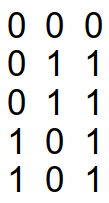
\includegraphics[width=0.1\textwidth]{Pics/sequences01_only} \\
                \caption{What is the value of $\hat{\theta}_W$?}
        \end{figure}

        \pause
        $\hat{\theta}_W = 3 / (1+1/2+1/3+1/4)=1.4$ \\
	but before we obtained $\hat{\theta}_T=1.6$. \\
	Why?
	
\end{frame}


\begin{frame}{Summary statistics}

	Possible summaries of DNA sequence data are:
	\begin{itemize}
		\item the number of segregating sites ($S$)
		\item the average number of pairwise differences ($\pi$)
	\end{itemize}
	but they don't provide much information regarding \textbf{allele frequencies}.

\end{frame}


\begin{frame}{The Site Frequency Spectrum (SFS)}

	\begin{block}{SFS}
	The SFS is obtained by tabulating the sample allele frequencies of all mutations.
	\end{block}

	\begin{columns}

                \column{0.2\textwidth}

                \begin{figure}
                        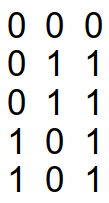
\includegraphics[width=0.6\textwidth]{Pics/sequences01_only}
                \end{figure}

                \column{0.8\textwidth}

		\pause

		The "1" alleles have frequencies $2/5$, $2/5$ and $4/5$.

		The proportions of "1" alleles with a frequency of $1/5$, $2/5$, $3/5$ and $4/5$
		in the sample are \pause $f_1=0$, $f_2=2/3$, $f_3=0$ and $f_4=1/3$.

                \begin{equation*}
                        \vec{f} = (f_1, f_2, ..., f_{n-1})
                \end{equation*}
		for a sample of $n$ haploid individuals.

        \end{columns}

\end{frame}


\begin{frame}{The Site Frequency Spectrum (SFS)}

        \begin{columns}

                \column{0.2\textwidth}

                \begin{figure}
                        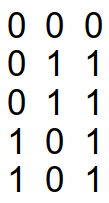
\includegraphics[width=0.6\textwidth]{Pics/sequences01_only}
                \end{figure}

                \column{0.8\textwidth}

		\begin{figure}
                        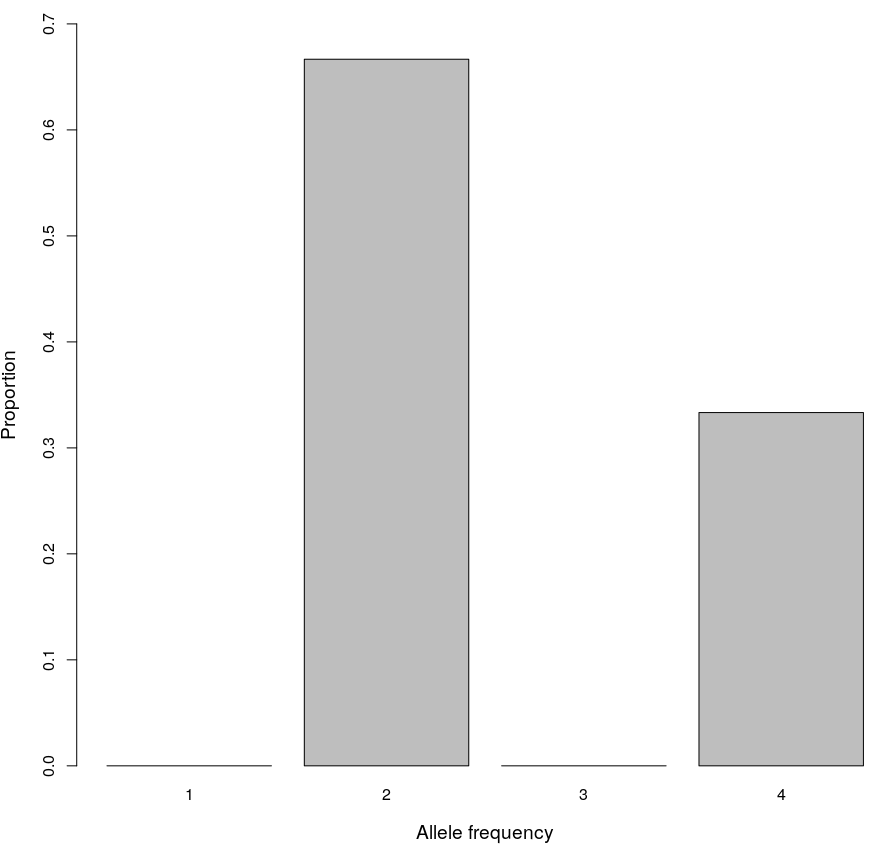
\includegraphics[width=0.75\textwidth]{Pics/SFS}
                \end{figure}

        \end{columns}

\end{frame}


\begin{frame}{Alleles}

	\small
	\begin{itemize}
		\item \textbf{ancestral} allele is the allele found in the MRCA of the sample.
		\item \textbf{derived} allele (or mutated) is an allele that is not ancestral.
	\end{itemize}

	\begin{figure}
        	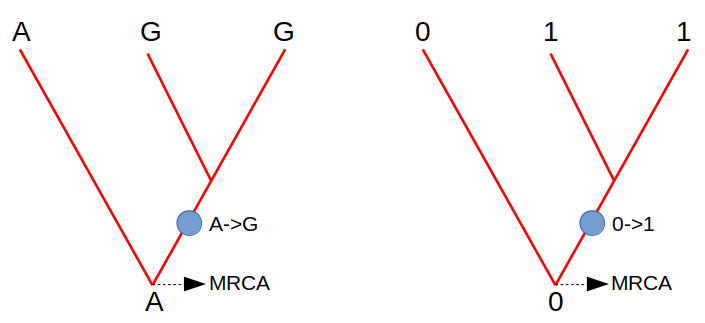
\includegraphics[width=0.8\textwidth]{Pics/ancder}
        \end{figure}

\end{frame}


\begin{frame}{Alleles}

	\bigskip
	\small
	The ancestral allele is often inferred using \textbf{outgroups}.
	
	e.g. if $C/T$ polymorphism in humans and primate have $C$, then $C$ is likely to be the ancestral allele.

	\begin{figure}
                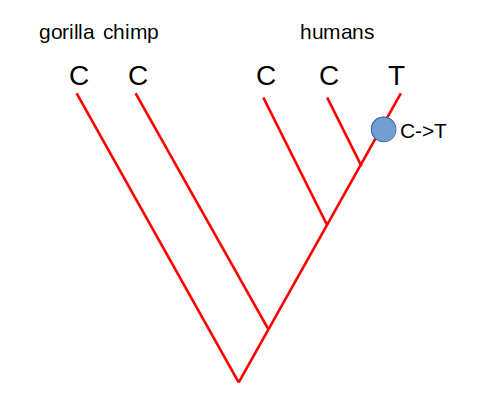
\includegraphics[width=0.5\textwidth]{Pics/ancder_species}
        \end{figure}

\end{frame}


\begin{frame}{Alleles}

        \begin{figure}
                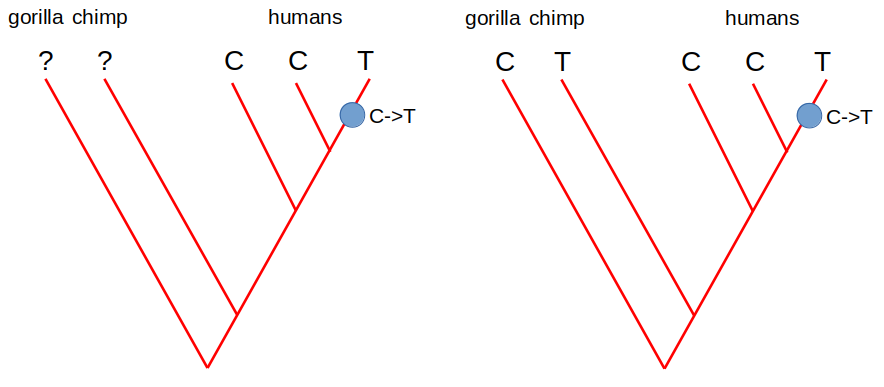
\includegraphics[width=0.9\textwidth]{Pics/ancder_unknown}
        \end{figure}

\end{frame}


\begin{frame}{The Site Frequency Spectrum (SFS)}

	If no information on the ancestral allele is available, we can \textit{fold} the frequency
	spectrum.
	\begin{block}{}
	The \textbf{folded frequency spectrum} $f^*$ is obtained by adding together the frequencies
	of the derived and ancestral alleles.
	\end{block}

	$f^* = f_i + f_{n-j}$ for $j<n/2$ and \\
	$f^* = f_j$ for $j=n/2$ \\
	only defined for values of $f^* \leq n/2$.

\end{frame}


\begin{frame}{The folded SFS}

        \begin{columns}

                \column{0.2\textwidth}

                \begin{figure}
                        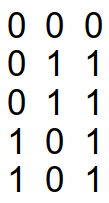
\includegraphics[width=0.6\textwidth]{Pics/sequences01_only}
                \end{figure}

                \column{0.8\textwidth}

		$\vec{f^*} = $ \pause $(f^*_1=1/3, f^*_2=2/3)$

        \end{columns}

\end{frame}


\begin{frame}{The Site Frequency Spectrum}

	\begin{itemize}
		\item $S$ and $\pi$ can be calculated directly from $\vec{f}$ but the opposite is not true.
		\item Alleles segregating at frequency of $1/n$ are called \textbf{singletons}.
		\item The expected SFS under the standard coalescence model with infinite sites mutations is
		\begin{equation}
			E[f_i] = \frac{1/j}{\sum_{k=1}^{n-1} \frac{1}{k}}
		\end{equation}
		with $j=1,2,...,n-1$
	\end{itemize}

	\bigskip
	\tiny jupyter-notebook: coalescence

\end{frame}


\begin{frame}{Tree shape and population size}

	\small
	Measured in number of generations, the expected coalescence time for $k$ lineages is $2N/[k(k-1)]$.

	\begin{figure}
         	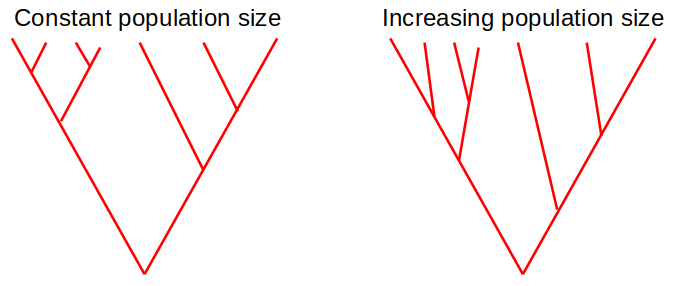
\includegraphics[width=0.85\textwidth]{Pics/tree_N_i}
        \end{figure}

\end{frame}


\begin{frame}{Tree shape and population size}

        \small
        Measured in number of generations, the expected coalescence time for $k$ lineages is $2N/[k(k-1)]$.

        \begin{figure}
                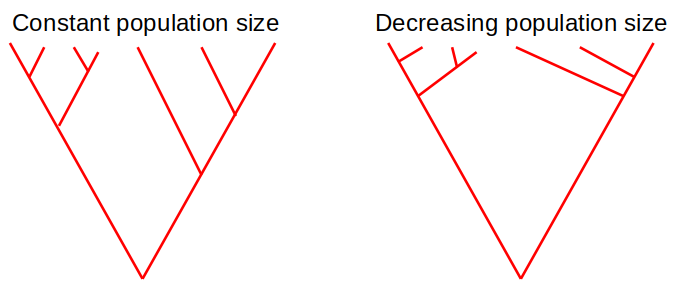
\includegraphics[width=0.85\textwidth]{Pics/tree_N_d}
        \end{figure}

\end{frame}


\begin{frame}{Intended Learning Outcomes}

        \underline{Coalescence theory}

        \bigskip

        In this lecture you have learnt to
        \begin{itemize}
                \item describe principles and assumptions of the coalescence theory
                \item discuss the infinite sites model
                \item provide estimators of $\theta$ and effective population sizes
		\item measure genetic variability with summary statistics and the site 
		frequency spectrum with \texttt{R}
        \end{itemize}

\end{frame}









